%-------------------------------------------------------------------------------
\chapter[General How-To?]{General How-To?}
%-------------------------------------------------------------------------------
\pagebreak
%...............................................................................
\section{Running a morphodynamics simulation: first steps}
%...............................................................................
The minimum set of files to run a morphodynamics simulation includes:
\begin{itemize}
\item the steering file(s) (text/ascii file \texttt{*.cas})
\item the geometry file (format selafin/binary \texttt{*.slf})
\item the boundary conditions file (text/ascii file \texttt{*.cli})
\item additional or optional input files as the fortran file (text/ascii file \texttt{*.f}), the reference file (format selafin/binary \texttt{*.slf}), etc.
\end{itemize}

Typically, these files are contained in a folder, for example in the folder {\texttt simulation\}:
\begin{footnotesize}
\begin{verbatim}
simulation\bc_bifurcation_tel.cli
simulation\geo_bifurcation.slf
simulation\res_bifurcation_hotstart_tel.slf
simulation\run_bifurcation_sis.cas
simulation\run_bifurcation_tel.cas
\end{verbatim}
\end{footnotesize}

Running a simulation from a Linux terminal:
\begin{footnotesize}
\begin{verbatim}
telemac2d.py run_bifurcation_tel.cas
\end{verbatim}
\end{footnotesize}

%...............................................................................
\subsection{Gaia's steering file (\texttt{*.cas})}
%...............................................................................
This file contains the necessary information for running a simulation, it also must include the values of parameters that are different from the default values (as specified in the dictionary file \texttt{gaia.dico}):
\begin{itemize}
\item Input and output files
\item Physical parameters (sand diameter, settling velocity, etc.)
\item Main sediment transport processes (transport mechanisms, closure relationships, etc.)
\item Additional sediment transport processes (secondary currents, slope effect, etc.)
\item Numerical options and parameters (numerical scheme, solvers, etc.)
\end{itemize}

\pagebreak

%-------------------------------------------------------------------------------
\subsubsection{Sketch of the gaia's steering file (\texttt{*.cas})}
%-------------------------------------------------------------------------------
\lstset{language=TelemacCas,
        basicstyle=\scriptsize\ttfamily}
\begin{lstlisting}[frame=trBL]
/----------------------------------------------------------------------/
/ gaia bedload                                                      /
/----------------------------------------------------------------------/
/
/----------------------------------------------------------------------/
/  FILES                                                               /
/----------------------------------------------------------------------/
/
/ --- GEOMETRY ---
GEOMETRY FILE				= '../geo_bifurcation.slf'
BOUNDARY CONDITIONS FILE		= '../bc_bifurcation_tel.cli'
/
/ --- RESULTS ---
RESULTS FILE				= 'res_bifurcation_gai.slf'
/
...
/----------------------------------------------
/  PHYSICAL PARAMETERS
/----------------------------------------------
/
BED LOAD                                   = YES
BED-LOAD TRANSPORT FORMULA FOR ALL SANDS   = 1
SEDIMENT DIAMETERS                         = 0.000120
/
...
/----------------------------------------------------------------------/
/  NUMERICAL PARAMETERS                                                /
/----------------------------------------------------------------------/
/
MASS-BALANCE                              = YES
SOLVER ACCURACY                           = 1.E-12
MASS-LUMPING                              = YES
...
\end{lstlisting}

%-------------------------------------------------------------------------------
\subsubsection{Examples of physical parameters in the Gaia's steering file}
%-------------------------------------------------------------------------------
\begin{itemize}
\item Sediment diameters, defined by the keyword \telkey{SEDIMENT DIAMETERS} (real list, {\ttfamily = 0.01} m by default)
\item Sediment density, defined by the keyword \telkey{SEDIMENT DENSITY} (real type, {\ttfamily = 2650.0} kg$/$m$^3$ by default)
\item Shields parameter $\tau_c$ [N\,m$^{-2}$], defined by the keyword \telkey{SHIELDS PARAMETERS} \textcolor{blue}{\sout{(real list, if not provided it is computed by \gaia{}}} \textcolor{blue}{(real list, = -9 by default). If it is not known, it is necessary to give a negative value to let \gaia{}} compute it as a function of the non-dimensional grain diameter $D_*=d_{50}[(\rho_s/\rho-1)g/\nu^2]^{1/3}$ in the subroutine \texttt{init\_sediment\_gaia.f}:
\begin{equation*}
\frac{\tau_c}{g(\rho_s -\rho)d_{50}}=\left\{\begin{array}{ll}
0.24 D_*^{-1}, & D_* \leq 4 \\
0.14 D_*^{-0.64}, & 4 < D_* \leq 10 \\
 0.04 D_*^{-0.10}, & 10 < D_* \leq 20\\
0.013 D_*^{0.29}, & 20 < D_* \leq 150 \\
0.045, & 150 \leq D_*
\end{array}
\right.
\end{equation*}
with $d_{50}$ the median sand grain diameter (m), $\rho$ the water density $=1000$ kg$/$m$^3$ by default, $\rho_s$ the sediment density $=2650$kg$/$m$^3$ by default, and $\nu$ the kinematic viscosity $=1.0\times 10^{-6}$m$^2$s$^{-1}$ by default.

\item Settling velocity, it can be specified by the user or calculated by the model as a function of grain diameter, keyword \telkey{SETTLING VELOCITIES } (real list, \textcolor{blue}{=-9 by default}). \textcolor{blue}{If a negative value is given, \gaia{} will compute it as function of grain diameter}:
  \begin{equation*}
w_{s} = \left\{\begin{array}{ll}
\displaystyle
\frac{(s-1)g d_{50}^2}{18\nu}, & \quad \text{if } d_{50} \leq 10^{-4} \\
\displaystyle
\frac{10\nu}{d_{50}} \left(\sqrt{1+0.01\frac{(s-1)gd_{50}^3}{\nu^2}}-1\right), & \quad \text{if } 10^{-4} \leq d_{50} \leq 10^{-3}\\
\displaystyle
1.1 \sqrt{(s-1)gd_{50}}, & \quad \text{otherwise}
\end{array}
\right.
\end{equation*}
with $s=\rho_{s}/\rho_0$ is the relative density and $g$ is the acceleration of the gravity.%
\item Bed porosity, keyword \telkey{NON COHESIVE BED POROSITY} (real type, {\ttfamily = 0.40} by default)
\end{itemize}



\subsection{Boundary conditions file}\label{sec:flags}
Thirteen variables for each boundary nodes are specified in the boundary condition file (usually named with extension \texttt{*.cli}). An example is given below:

\begin{lstlisting}[frame=trBL]
5 4 4 0.0 0.0 0.0 0.0 4 0.0 0.0 0.0 565 1
5 4 4 0.0 0.0 0.0 0.0 4 0.0 0.0 0.0 564 2
5 4 4 0.0 0.0 0.0 0.0 4 0.0 0.0 0.0 563 3
5 4 4 0.0 0.0 0.0 0.0 4 0.0 0.0 0.0 562 4
5 4 4 0.0 0.0 0.0 0.0 4 0.0 0.0 0.0 561 5
5 4 4 0.0 0.0 0.0 0.0 4 0.0 0.0 0.0 560 6
\end{lstlisting}

Each column is named after a flag, as follows:
\subsubsection{\telemac{2D}}
\begin{lstlisting}[frame=trBL]
LIHBOR LIUBOR LIVBOR HBOR UBOR VBOR AUBOR LITBOR TBOR ATBOR BTBOR N K
\end{lstlisting}
\subsubsection{\gaia{}}
\begin{lstlisting}[frame=trBL]
LIHBOR LIQBOR LIVBOR Q2BOR UBOR VBOR AUBOR LIEBOR/LICBOR EBOR/CBOR ATBOR BTBOR N K
\end{lstlisting}
%\begin{center}
%\begin{small}
%\texttt{\textcolor{black}{LIHBOR}, \textcolor{black}{LIUBOR/LIQBOR}, \textcolor{black}{LIVBOR}, \textcolor{black}{HBOR}, \textcolor{black}{VBOR}, \textcolor{black}{UBOR}, \textcolor{black}{VBOR}, \textcolor{black}{CHBORD}, \textcolor{black}{LITBOR/LIEBOR/LICBOR}, COL10, COL11, G, L}
%\end{small}
%\end{center}
where \texttt{N, K} are respectively the global and local boundary node numeration. Flags \texttt{ATBOR, BTBOR} are discussed in the \telemac{2D} user manual. For both modules \telemac{2D} and \gaia{}, flags can be specified as follows:
\begin{itemize}
\item \texttt{\textcolor{black}{=2:}} closed boundary (wall)
\item \texttt{\textcolor{black}{=4:}} free boundary (Neumann's type)
\item \texttt{\textcolor{black}{=5,6:}} imposed value (Dirichlet's type)
\end{itemize}

The different types of boundaries are (integer variables):
\subsubsection{\telemac{2D}}
\begin{itemize}
\item \texttt{\textcolor{black}{LIHBOR:}} flag to set the water depth (\texttt{=5})
\item \texttt{\textcolor{black}{LIUBOR:}} flag to set the discharge (\texttt{=5}) or the velocity (\texttt{=6}) in the $x-$direction
\item \texttt{\textcolor{black}{LIVBOR:}} flag to set the discharge (\texttt{=5}) or the velocity (\texttt{=6}) in the $y-$direction
\item \texttt{\textcolor{black}{LITBOR:}} flag to set the tracer
\end{itemize}
For further details see the \telemac{2D}'s reference manual.
\subsubsection{\gaia{}}
\begin{itemize}
\item \texttt{\textcolor{black}{LIEBOR:}} flag to set the bottom elevation
\item \texttt{\textcolor{black}{LICBOR:}} flag to set the equilibrium or imposed concentration
  \item \texttt{\textcolor{black}{LIQBOR:}} flag to set the imposed bedload discharge
\end{itemize}

Values (real variables) can be specified as follows:
\subsubsection{\telemac{2D}}
\begin{itemize}
\item \texttt{\textcolor{black}{HBOR:}} prescribed water depth
\item \texttt{\textcolor{black}{UBOR:}} prescribed discharge or velocity in the $x-$direction
\item \texttt{\textcolor{black}{VBOR:}} prescribed discharge or velocity in the $y-$direction
\item \texttt{\textcolor{black}{AUBOR:}} friction coefficient on lateral walls
\end{itemize}
\subsubsection{\gaia{}}
\begin{itemize}
\item \texttt{\textcolor{black}{EBOR:}} prescribed bed evolution
\item \texttt{\textcolor{black}{CBOR:}} prescribed concentration
\item \texttt{\textcolor{black}{Q2BOR:}} prescribed bedload discharge, expressed in m$^2/$s excluding voids.
\end{itemize}

For the particular case where a bedload solid discharge is imposed, an extra boundary condition file needs to be defined for \gaia{}. The treatment of boundary conditions for bedload and suspended sediment transport is given in \S\ref{sec:BedloadTransport} and \S\ref{sec:SuspendedSedimentTransport}, respectively.

%...............................................................................
\subsubsection{Coupling hydrodynamics and morphodynamics: sketch of the Telemac-2d's steering file with the required keywords}
%...............................................................................
\lstset{language=TelemacCas,
        basicstyle=\scriptsize\ttfamily}
\begin{lstlisting}[frame=trBL]
...
INITIAL TIME SET TO ZERO                = YES
TIME STEP			        = 20.0
NUMBER OF TIME STEPS                    = 100000
...
/----------------------------------------------------------------------/
/  COUPLING WITH GAIA                                                  /
/----------------------------------------------------------------------/
/
COUPLING WITH                            = 'GAIA'
GAIA STEERING FILE                    = 'run_bifurcation_gai.cas'
/
/---------------------------------------------------------------------
/ INITIAL CONDITIONS
/---------------------------------------------------------------------
/
COMPUTATION CONTINUED             = YES
PREVIOUS COMPUTATION FILE         = 'res_bifurcation_hotstart_tel.slf'
...
\end{lstlisting}
%...............................................................................
\subsection{Fortran files (\texttt{*.f})}
%...............................................................................
Programming can be necessary for particular applications. A Fortran file (keyword \telkey{FORTRAN FILE}) can be specified in the \telemac{2D} or \telemac{3D} or \gaia steering file with the required subroutine(s). \textcolor{blue}{\sout{In case of coupling}} All subroutines (\gaia subroutines also) can be incorporated in the \telemac fortran file. Is is also possible to have a \telemac and a \gaia fortran file. Be aware, if there is no \telemac{2D} or \telemac{3D} fortran file, the \gaia fortran file will not taken into account.
Some common applications are given below:
\begin{itemize}
\item \textbf{Definition of rigid areas:} \texttt{bed\_init\_user.f} is used for specifying the rigid areas. \textcolor{blue}{\sout{The position of the non-erodable areas (array \texttt{ZR}) are imposed in this subroutine}}\textcolor{blue}{The thickness of the erodable area (array \texttt{ESTRATUM}) is imposed in this subroutine}

\item \textbf{New sediment transport formula}: \texttt{qsform\_gaia.f} can be used to program a sediment transport formula that is different from those already implemented in \gaia{}

\item \textbf{Replace data from a result file}: \texttt{condim\_gaia.f} can be used for \textcolor{blue}{\sout{reading}} \textcolor{blue}{replacing} data from a results file computed from a simulation performed for example from the waves module \tomawac{}

\end{itemize}

\gaia{}'s main subroutines are found in the folder \texttt{/sources/gaia/} of the \telemacsystem{}. Please note that if there is no fortran file specified in \telemac{2D} or \telemac{3D}, then \gaia's fortran file must be specified in the \telemac{2D} or \telemac{3D} steering file.

\pagebreak

%-------------------------------------------------------------------------------
\subsubsection{Graphical printouts}
%-------------------------------------------------------------------------------
The keyword \telkey{VARIABLES FOR GRAPHIC PRINTOUTS} can include a variety of output variables to be printed in the results file (character list, set to {\ttfamily = U,V,H,S,B,E} by default). The graphic and listing printout periods are the same as in the \telemac{2D} or \telemac{3D} computation. The list of variables that can be printed in the \gaia{}'s results file is \textcolor{blue}{CHANGE THIS PART WHEN DEVELOPMENTS WILL BE FINISHED}:
\begin{lstlisting}[frame=trBL]
U="velocity along x axis (m/s)";
V="velocity along y axis (m/s)";
C="wawe celerity (m/s)";
H="water depth (m)";
S="free surface elevation (m)";
B="bottom elevation (m)";
F="Froude number";
Q="scalar flowrate of fluid (m2/s)";
I="flowrate along x axis (m2/s)";
J="flowrate along y axis (m2/s)";
M="bed-load discharge (m2/s)";
N="bed-load discharge along x axis (m2/s)";
P="bed-load discharge along y axis (m2/s)";
E="bottom evolution (m)";
R="non erodable bottom";
KS="total bed roughness (m)";
TOB="Bed Shear stress (Totalfriction) (N/m2)";
MU = "Skin friction correction factor";
D50 = "Mean grain diameter";
THETAW="wave angle with axis Oy (deg)";
QSSUSP="suspended load transport rate (m2/s)";
QSBL="bed load transport rate (m2/s)";
W="wave height";
X="wave period";
UWB="wave orbital velocity (m/s)";
1Ai="fraction of sediment of class i in the first layer";
2Ai="fraction of sediment of class i in the second layer";
kAi="fraction of sediment of class i in the k layer";
kES="thickness of the k layer";
kCONC="concentration of bed layer k";
QSi="bed load transport rate of sediment of class i";
CSi="concentration volumic or mass concentration for class i";
CSAT="saturated concentration (kg/m3)";
A="supplementary variable A";
G="supplementary variable G";
L="supplementary variable L";
O="supplementary variable O"
\end{lstlisting}

The graphical printout period is controlled in the \telemac{2D} steering file through the keyword \telkey{GRAPHIC PRINTOUT PERIOD} (integer type, {\ttfamily = 1} by default).
Similarly, the keyword \telkey{LISTING PRINTOUT PERIOD} (integer type, {\ttfamily = 1} by default) controls the printout period on the screen.

%-------------------------------------------------------------------------------
\section{Compute sediment fluxes through a given section(s)}
%-------------------------------------------------------------------------------
Use the keywords {\ttfamily FLUXLINE} (logical type, set to {\ttfamily NON} by default) and {\ttfamily FLUXLINE INPUT FILE} (character type).

The format of the {\ttfamily FLUXLINE INPUT FILE} includes (see Figure~\ref{fig:fluxline_example}):
\begin{itemize}
\item The number of fluxlines (integer)
\item The definition of the fluxlines, given by:
  \begin{itemize}
  \item The specification of two points of the fluxline (\texttt{fluxline\_x1, fluxline\_y1, fluxline\_x2, fluxline\_y2}), followed by
  \item the definition of the bounding box (\texttt{box\_x1, box\_y1, box\_x2, box\_y2})
  \item An integer (value not used)
  \end{itemize}
\end{itemize}

An example of the {\ttfamily FLUXLINE INPUT FILE} is given below:

\begin{lstlisting}[frame=trBL]
5
94.0   31.2  99.0  31.2 95.0  31.0  98.0  31.6 1
94.0   42.5  99.0  42.5 96.0  42.0  98.0  43.0 1
101.0  42.5  107.0 42.5 104.0 42.0  106.0 43.0 1
101.0  31.2  107.0 31.2 104.0 31.0  106.0 31.6 1
100.0  45.0  102.0 48.0 100.0 46.0  102.0 47.5 1
\end{lstlisting}

\begin{figure}[H]
\begin{center}
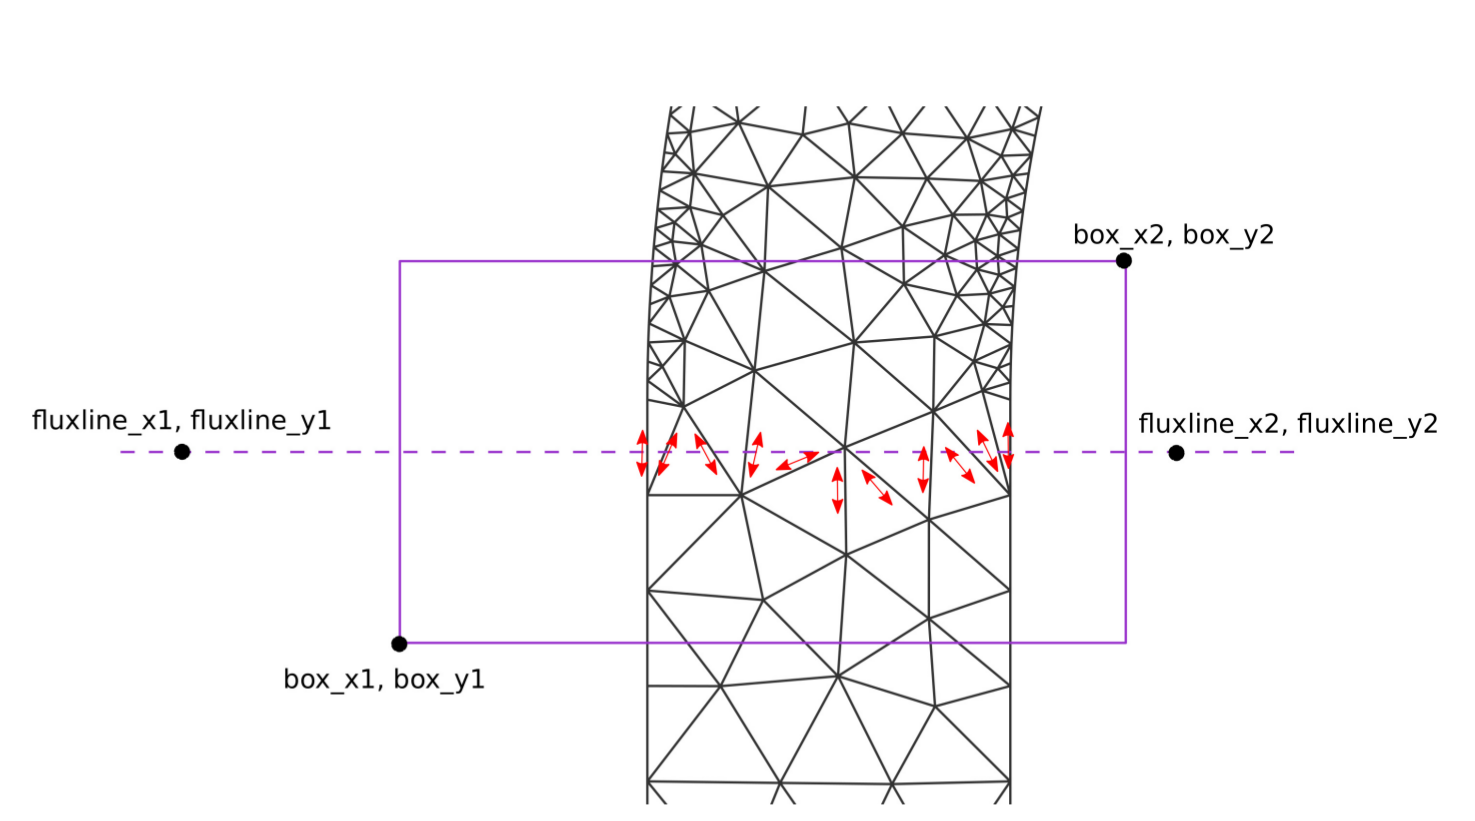
\includegraphics[scale=0.25,angle=0]{graphics/fluxline_example.png}
\caption{Description of a single fluxline and edge fluxes (red).}\label{fig:fluxline_example}
\end{center}
\end{figure}

Further details can be found in Stadler L. (2015) \textit{Calculating correct water and sediment fluxes in TELEMAC2D and GAIA}. Proceedings of the 22$^{th}$
Telemac \& Mascaret User Club, STFC Daresbury Laboratory, UK, 13-16 October.

%\pagebreak
%-------------------------------------------------------------------------------
\section{Implement a new bedload transport formula}
%-------------------------------------------------------------------------------
To implement a new bedload transport formula, the keyword {\ttfamily BED-LOAD TRANSPORT FORMULA} must be set to {\ttfamily = 0}. The Fortran subroutine must be added into the fortran file of \textsc{Telemac-2d} or \textsc{Telemac-3d}, keyword {\ttfamily FORTRAN FILE}.

The template subroutine is called \texttt{qsfrom.f} and can be found in the folder \texttt{/sources/gaia}
\begin{lstlisting}[frame=trBL]
!                    *****************
                     SUBROUTINE QSFORM
!                    *****************
     &(U2D, V2D, TOB, HN, XMVE, TETAP, MU, NPOIN, DM,
     & DENS, GRAV, DSTAR, AC, QSC, QSS)
!
!***********************************************************************
! GAIA   V6P2                                   21/07/2011
!***********************************************************************
!
!brief    ALLOWS THE USER TO CODE THEIR OWN BEDLOAD TRANSPORT
!+                FORMULATION, BEST SUITED TO THEIR APPLICATION.
!
!~~~~~~~~~~~~~~~~~~~~~~~~~~~~~~~~~~~~~~~~~~~~~~~~~~~~~~~~~~~~~~~~~~~~~~~
!~~~~~~~~~~~~~~~~~~~~~~~~~~~~~~~~~~~~~~~~~~~~~~~~~~~~~~~~~~~~~~~~~~~~~~~
!
      USE INTERFACE_GAIA, EX_QSFORM => QSFORM
!     USE DECLARATIONS_GAIA
      USE BIEF
      IMPLICIT NONE
      INTEGER LNG,LU
      COMMON/INFO/LNG,LU
!
!+-+-+-+-+-+-+-+-+-+-+-+-+-+-+-+-+-+-+-+-+-+-+-+-+-+-+-+-+-+-+-+-+-+-+-+
!
      TYPE(BIEF_OBJ),   INTENT(IN)    :: U2D,V2D,TOB,HN,TETAP,MU
      TYPE(BIEF_OBJ),   INTENT(INOUT) :: QSC, QSS
      INTEGER,          INTENT(IN)    :: NPOIN
      DOUBLE PRECISION, INTENT(IN)    :: XMVE, DM, DENS, GRAV, DSTAR, AC
!
!+-+-+-+-+-+-+-+-+-+-+-+-+-+-+-+-+-+-+-+-+-+-+-+-+-+-+-+-+-+-+-+-+-+-+-+
!
!
      INTEGER          :: I
      DOUBLE PRECISION :: C1, C2, T
      DOUBLE PRECISION, PARAMETER :: ACOEFF = 0.004D0!Sediment transport param (m^2s^-1)
!
!======================================================================!
!======================================================================!
!                               PROGRAM                                !
!======================================================================!
!======================================================================!
!
!     GRASS (1981) TYPE
!
      DO I = 1, NPOIN

        QSC%R(I) = ACOEFF * U2D%R(I) * (U2D%R(I)**2+V2D%R(I)**2) ! 1D Grass (1981)
        QSS%R(I) = 0.D0                                          ! Zero suspended load

      END DO
!
!
!-----------------------------------------------------------------------
!
      RETURN
      END
\end{lstlisting}

%\pagebreak
%-------------------------------------------------------------------------------
%\section{Define a rigid bed}
%-------------------------------------------------------------------------------
%TODO
%\subsection{Data from selafin file}
%\subsection{Data coded by the user in the fortran file}

%\pagebreak
%-------------------------------------------------------------------------------
\section{Print a new output variable in the selafin file}
%-------------------------------------------------------------------------------
\begin{itemize}
\item Declare the {\ttfamily PRIVE} variable, for example as:

{\ttfamily USE DECLARATIONS\_gaia, ONLY : PRIVE}

\item Use the following expression to include the variable you want to visualize:

{\ttfamily PRIVE\%ADR(N)\%P\%R(K) = [Here the variable you want to visualize]}, where {\ttfamily N} is the number of variables that you want to visualize and {\ttfamily K} is the number of nodes.

\item In the \gaia's steering file you can use the flags {\ttfamily'A'} or {\ttfamily'G'} to visualize the {\ttfamily PRIVE} variable, for example as:

{\ttfamily VARIABLES FOR GRAPHIC PRINTOUTS='U,V,S,H,B,Q,M,E,QSBL,TOB,MU,A'}
\end{itemize}

The default name {\ttfamily PRIVE 1} (for {\ttfamily N=1}) can be modified in the subroutine {\ttfamily nomvar\_gaia.f}.

\begin{lstlisting}[frame=trBL]
DO K=1, NPOIN
  PRIVE%ADR(1)%P%R(K) = [variable to visualize]
ENDDO
\end{lstlisting}

%\pagebreak
%-------------------------------------------------------------------------------
\section{Introduce a new keyword}
%-------------------------------------------------------------------------------
\begin{itemize}
\item In {\ttfamily declarations\_gaia.f} declare the variable to be called from a keyword e.g. {\ttfamily HMIN\_BEDLOAD}
\item In {\ttfamily lecdon\_gaia.f} declare .... {\ttfamily HMIN\_BEDLOAD=MOTREA(ADRESS(2,52))}
\item Declaration in the modified subroutine through {\ttfamily USE DECLARATIONS\_GAIA, ONLY : HMIN\_BEDLOAD}
\end{itemize}


%\pagebreak
%-------------------------------------------------------------------------------
\section{Read and use a variable from a selafin file}
%-------------------------------------------------------------------------------
Case of spatially distributed sediment zones

\begin{itemize}
\item Create the different zones with, e.g. BlueKenue
\item Add in your steering file:
  \begin{lstlisting}[frame=trBL]
NUMBER OF PRIVATE ARRAYS = 1
NAMES OF PRIVATE VARIABLES= 'ZONE                            '
\end{lstlisting}
(32 characters)%\textvisiblespace\textvisiblespace\textvisiblespace
\item Modify the subroutine \texttt{init\_compo.f}, for example:
\begin{lstlisting}[frame=trBL]
      DO J=1,NPOIN
      NCOUCHES(J)=1
	  IF(PRIVE%ADR(1)%P%R(J).EQ.1.D0) THEN
	  AVAIL(J,1,1)=1.D0
	  AVAIL(J,1,2)=0.D0
	  ELSEIF(PRIVE%ADR(1)%P%R(J).EQ.2.D0) THEN
	  AVAIL(J,1,1)=0.D0
	  AVAIL(J,1,2)=1.D0
	  ELSE
	  AVAIL(J,1,1)=0.5D0
	  AVAIL(J,1,2)=0.5D0
	  ENDIF
      ENDDO
\end{lstlisting}
\end{itemize}


%\pagebreak
%-------------------------------------------------------------------------------
%\section{Define the soil stratigraphy (init\_compo)}
%-------------------------------------------------------------------------------
%TODO

%\pagebreak
%-------------------------------------------------------------------------------
%\section{Suppress bed updating}
%-------------------------------------------------------------------------------
%Set \telkey{STATIONARY MODE = YES} (logical type, set to {\ttfamily = NO} by default)

%\pagebreak
%-------------------------------------------------------------------------------
\section{Using a non-declared variable in a Gaia's subroutine}
%-------------------------------------------------------------------------------
If you want to use, for example, parameter \texttt{NPTFR} and the table \texttt{NBOR(NPTFR)} in the subroutine NOEROD,
declare:

\texttt{USE DECLARATIONS\_GAIA, ONLY : NPTFR, MESH}

\texttt{INTEGER, POINTER :: NBOR(:)}

Then the following alias can be declared:

\texttt{NBOR=>MESH\%NBOR\%I}

%\pagebreak
%-------------------------------------------------------------------------------
\section{Prevent erosion when water depth is smaller than a threshold value}
%-------------------------------------------------------------------------------
At for example intertidal wetlands with flooding and drying or tidal areas, the bottom friction could be very high when the water depth is very small, even for small velocities, leading to high and unphysical erosion rates. To prevent that, the keyword \telkey{MINIMAL VALUE OF THE WATER HEIGHT} can be used (the value by default is $1.0 \times 10^{-3}$m). This keyword is activated when \telkey{TIDAL FLATS = YES}.

%\pagebreak
%-------------------------------------------------------------------------------
\section{Set a non-erodible bottom}
%-------------------------------------------------------------------------------
\subsection{By defining a variable in the geometry file (e.g. BlueKenue)}
\begin{enumerate}
\item Create a new variable in your geometry file, for example \texttt{NOER}
\item Set the following keywords in the \gaia steering file:
\begin{lstlisting}[frame=trBL]
NUMBER OF PRIVATE ARRAYS = 1
NAMES OF PRIVATE VARIABLES= 'NOER            M               '
\end{lstlisting}
\item The above private variable can be accessed via the \texttt{PRIVE} structure, for example with the \texttt{PRIVE\%ADR(1)\%P\%R} for the (private) variable number $1$.
\item Modify the subroutine \texttt{noerod.f} as follows:
  \begin{itemize}
    \item Add the following line just below \texttt{USE BIEF}:
      \begin{lstlisting}[frame=trBL]
        USE DECLARATIONS_GAIA, ONLY: PRIVE
      \end{lstlisting}
    \item Replace for example the default \texttt{CALL OV} that sets the erodible bed 100 m below the river bottom \texttt{CALL OV('X=Y+C   ',ZR,ZF,ZF,-100.D0,NPOIN)} by the following:
      \begin{lstlisting}[frame=trBL]
       CALL OV('X=Y-Z   ',ZR,ZF,PRIVE%ADR(1)%P%R,0.D0,NPOIN)
      \end{lstlisting}
  \end{itemize}
\item Don't forget to call this subroutine from the keyword \texttt{FORTRAN FILE} in the steering file
\end{enumerate}

 \begin{WarningBlock}{Warning:}
The \texttt{X=Y-Z} function, here it works when \texttt{NOER} (that is to say \texttt{PRIVE\%ADR(1)\%P\%R}) is the \textbf{thickness of the erodible bed}, not the elevation of the non-erodible bed.
 \end{WarningBlock}

 \subsection{Non-erodible bed everywhere}
Replace in \texttt{noerod.f} the line of code:
\begin{lstlisting}[frame=trBL]
  CALL OV('X=Y+C   ',ZR,ZF,ZF,-100.D0,NPOIN)
\end{lstlisting}
with
\begin{lstlisting}[frame=trBL]
\texttt{CALL OV('X=Y+C   ',ZR,ZF,ZF,0.D0,NPOIN)}
\end{lstlisting}


{\footnotesize Thanks to Pilou1253, Jos\'e Diaz and Costas (Cyamin) for this contribution in the Forum}

%\pagebreak
%-------------------------------------------------------------------------------
\section{Modify the bottom from the subroutine corfon}
%-----------------------------------------------------------------------------
For example, you want to set the bottom at node $325$ equal to $2.1$ m
\begin{itemize}
\item Sequential: \texttt{ZF\%R(325)=2.1D0}
\item Parallel: \texttt{ZF\%R(GLOBAL\_TO\_LOCAL\_POINT(325,MESH))=2.1D0}
\end{itemize}

If there are several nodes to be modified, use a loop.

{\footnotesize Thanks to JMH (post \#9747)}

%-------------------------------------------------------------------------------
\section{Set-up a graded sediment problem with only one layer}
%-----------------------------------------------------------------------------
It is not possible to have only 1 layer for the graded sediments (see \texttt{init\_sediment.f}: the second layer is hard coded e.g. \texttt{AVAIL(J,2,K)}). So you need to initialise at least 2 layers. For the conservation example only 1 layer is needed, so the active layer thickness must be larger than the first layer $+$ the expected sedimentation. You can get this with no definition of active layer, because the default value is \texttt{1000}. And the last layer must be initialise by zero (which was missing), while the first layer must be initialised by \texttt{ZF-ZR}. As long as the active layer thickness is bigger than the first layer, no exchange with the 2nd layer will occur.

{\footnotesize Thanks to Rebekka Kopmann}


